%%%%%%%%%%%%%%%%%%%%%%% file template.tex %%%%%%%%%%%%%%%%%%%%%%%%%
%
% This is a general template file for the LaTeX package SVJour3
% for Springer journals.          Springer Heidelberg 2010/09/16
%
% Copy it to a new file with a new name and use it as the basis
% for your article. Delete % signs as needed.
%
% This template includes a few options for different layouts and
% content for various journals. Please consult a previous issue of
% your journal as needed.
%
%%%%%%%%%%%%%%%%%%%%%%%%%%%%%%%%%%%%%%%%%%%%%%%%%%%%%%%%%%%%%%%%%%%
%
% First comes an example EPS file -- just ignore it and
% proceed on the \documentclass line
% your LaTeX will extract the file if required
\begin{filecontents*}{example.eps}
%!PS-Adobe-3.0 EPSF-3.0
%%BoundingBox: 19 19 221 221
%%CreationDate: Mon Sep 29 1997
%%Creator: programmed by hand (JK)
%%EndComments
gsave
newpath
  20 20 moveto
  20 220 lineto
  220 220 lineto
  220 20 lineto
closepath
2 setlinewidth
gsave
  .4 setgray fill
grestore
stroke
grestore
\end{filecontents*}
%
\RequirePackage{fix-cm}
%
%\documentclass{svjour3}                     % onecolumn (standard format)
%\documentclass[smallcondensed]{svjour3}     % onecolumn (ditto)
\documentclass[smallextended]{svjour3}       % onecolumn (second format)
%\documentclass[twocolumn]{svjour3}          % twocolumn
%
\smartqed  % flush right qed marks, e.g. at end of proof
%
\usepackage{graphicx}
\usepackage{xcolor} % added by Zhiyuan
\usepackage{amsfonts} % added by ZHiyuan
\usepackage{amsmath}
\usepackage{algorithm}
\usepackage{algorithmic}
\usepackage{multicol}
\usepackage{frame}
\usepackage{wrapfig}
%
% \usepackage{mathptmx}      % use Times fonts if available on your TeX system
%
% insert here the call for the packages your document requires
%\usepackage{latexsym}
% etc.
%
% please place your own definitions here and don't use \def but
% \newcommand{}{}
%
% Insert the name of "your journal" with
% \journalname{myjournal}
%
\begin{document}

\title{A review of LSPI and improvement KLSPI%\thanks{Grants or other notes
%about the article that should go on the front page should be
%placed here. General acknowledgments should be placed at the end of the article.}
}
%\subtitle{Do you have a subtitle?\\ If so, write it here}

%\titlerunning{Short form of title}        % if too long for running head

\author{Zhiyuan Hu         
         %etc.
}

%\authorrunning{Short form of author list} % if too long for running head

\institute{Zhiyuan Hu \at
              TU Darmstadt \\
              Tel.: +123-45-678910\\
              Fax: +123-45-678910\\
              \email{zhiyuan.hu@stud.tu-darmstdat.de} \\
}

\date{Received: date / Accepted: date}
% The correct dates will be entered by the editor

\newcommand\myworries[1]{\textcolor{red}{#1}}
%\renewcommand\myworries[1]{}

\newcommand\vecPhi {\vec{\Phi}}

\maketitle

\begin{abstract}
TD method is widely used in reinforcement learning problem. In this article we review an important algorithm of TD method -- LSPI algorithm. Meanwhile, we discuss
some issues  of LSPI  like improvement variants, regularization, feature selection and numerical stability. The choice of feature is a fundamental problem of LSPI. To solve this problem we discuss the kernelized LSPI algorithm. Using ALD analysis, KLSPI uses an automatically constructed subset of sample dataset to calculate kernel, which could keep the generalization ability without huge loss of precision.


\keywords{LSPI \and LSTD \and KLSPI \and Kernel Machine}
% \PACS{PACS code1 \and PACS code2 \and more}
% \subclass{MSC code1 \and MSC code2 \and more}
\end{abstract}

\section{Introduction}
\label{intro}

Reinforcement Learning (RL) attracts many research interests not only in machine learning but also in many other disciplines like finance, robotic or optimal control \cite{kaelbling1996reinforcement}. RL Approaches give an exciting prospect since they are generic, highly automated and could be model-free \cite{rajeswaran2017towards}. 
%Traditionally there are two approaches to solve RL problem, gradient method to find optimal policy directly or estimate value function to obtain optimal policy indirectly. 
In this paper we focus on the method of value function estimation, which could be split mainly into three classe: (i) dynamic programming (DP) including policy iteration and value iteration, (ii) temporal difference (TD) methods such as TD ($\lambda$), Q-learning and (iii)  rollout-based Monte Carlo method \cite{kober2013reinforcement}.\\
This paper mainly focus the least square policy iteration algorithm (LSPI) and its variants, which combine (i) and (ii). DP is the basic algorithm for RL problem but not practical in complex real world system since DP requires the state transition model and reward model, which is normally unknown. 
%Another drawback is that DP requires that both action and state should be discrete, otherwise only limited situation such like LQR(linear quadratic regulator) case could be solved. 
\\
TD methods compute value functions, or approximations of these. The unique thing is that it try to minimize the error of temporal  consecutive predictions instead of an overall
prediction error \cite{kunz2000introduction}, which is very similar to dopamine mechanism in animal brain \cite{glimcher2011understanding}. LSTD methods are an enhancement of original TD methods, using mean squared error instead of gradient descent to minimize the error of gradient. This approach is very time-efficient in comparison to TD methods and it doesn't require learning rate.
\\
LSPI algorithm integrate LSTD method into Policy Iteration, using LSTD method to linearly approximate  action-value function Q(s, a) and using Bellman equation to update policy. In comparison to non linear approaches, it could directly compute close form solution and provide convergence guarantees. Meanwhile, in comparison to dynamic programming, it does not limit state-space to be discrete, and, in comparison to TD methods, the sample data could come from an arbitrary policy. \\
Feature selection is a fundamental problem of LSPI. The performance of algorithm highly depends on the quality of manually designed features. Kernel methods is widely used as a non-parametric method to solve feature engineering problem. KLSPI use kernel methods to avoid feature design and use approximate linear dependency(ALD) analysis to decrease the dataset for kernel methods.

\section{Problem Statement \& Notation}
\label{sec:problem_state}
\subsection{Markov Decision Process}
\label{sec:problem_MDP}
In this paper we consider the problem as  discrete-time \textit{Markov Decision Process}(MDP).
An MDP could be represented as a tuple, $\{S, A, R, P, \gamma \}$, where $S$ is the state space, $A$ is the action space, $P$ is the probabilistic transition model, where $P(s_t' \vert s_t, a_t)$ is the probability from state $s_t$ to state $s_t '$ with taking action $a_t$ at time step t, and R is the reward function $ R: S \times A \times S \rightarrow \mathbb{R} $, such that $R(s, a, s')$ represents the reward obtained when taking action a in state s and ending up in state s'. The $\gamma \in [0, 1] $  denotes a discount factor, for discounting future rewards. If the sequence of states will end in a terminating state or absorbing state, it would be called as episodic. If the terminating state will be reached in a fixed number length, it could be called as finite-horizon task. In infinite-horizon task the length of an episode is infinite without termination.\\
Significant property of MDP is that the future state only depends on the current state of system \cite{sutton1998introduction},
$
P({s_{t+1}}, r_{t+1} \vert s_t, a_t, r_t, s_{t-1}, a_{t-1}, r_{t-1}, ..., s_0, a_0 ) = P(s_{t+1} , r_{t+1} \vert s_t, a_t)
$.
Therefore the general case that the probability distribution of future states is a function of all past states could be simplified as function of last state and action.
 


%The Policy of MDP is defined as a function $\pi: S \rightarrow Pr(A)$, where $Pr(A)$ is a probability distribution in the action space. Policy could be deterministic or stochastic. The objective is to find the optimal policy $\pi^*$ to maximize the discounted total reward $J_\pi$:
%\begin{align}
%J_{\pi^*} = \max_\pi {J_\pi} = \max_\pi \mathbb{E}_\pi [ \sum_{t=0}^\infty \gamma^t r_t]
%\end{align}





\subsection{Dynamic Programming, policy iteration and value iteration}
When we regard the reinforcement learning as a constrained optimization problem, we could derivative state-value function $V^{\pi}(s)$ and action-value function $Q^{\pi}(s, a)$\cite{gordon1999approximate}\cite{puterman2014markov}. Both of them give information about the quality of a state in order to find an optimal policy. They are formally defined as 
$V^\pi (s)$  $ = \mathbb{E}_\pi [ R_T \vert s_t = s] = \mathbb{E}_\pi [ {\sum_{k=0}^{\infty}\gamma^k r_{t+k} \vert s_t = s} ] \label{equ:origin:V}$, 
$Q_\pi(s, a) = \mathbb{E}_\pi [R_T \vert s_t = s, a_t = a] =  \mathbb{E}_\pi [ {\sum_{k=0}^{\infty}\gamma^k r_{t+k} \vert s_t = s, a_t = a} ] \label{equ:origin:Q}
$. Which leads to Monto-Carlo(MC) Methods \cite{boyan1999least}. 
%The connection between Q and V is displayed by
%$
%V^{\pi}(s) = \mathbb{E}_\pi[ Q^\pi(s, a)] = \sum_a \pi(s, a) Q^{\pi}(s, a)
%$.
$V^\pi$ denotes a mean expectation of the future reward over all possible actions a, weighted by the probability distribution of action $\pi(a|s)$. $Q^\pi$
represents an actual reward for a fixed choice of actions.
%$R_t = \sum_{i=t}^{T-1}R_{i+1} = r_{t+1} + \gamma r_{t+2} + \gamma^2 r_{t+3} + ... + \gamma^{T-t-1} r_T$. 
However, more practically we use the incremental form: 
\begin{align}
V^\pi(s) &= \sum_a \pi(a \vert s) \sum_{s'} P(s' \vert s, a) [r(s, a) + \gamma V^{\pi}(s')] \label{equ:V} \\
Q^\pi(s, a) &= r(s, a) + \gamma \sum_{s'} \sum_{a'} P(s' \vert a, s) \pi(a' \vert s') Q^\pi(s', a'). \label{equ:Q}
\end{align} 
\begin{wrapfigure}{r}{0.3\textwidth}	
	\centering
	\vspace{-15pt}
	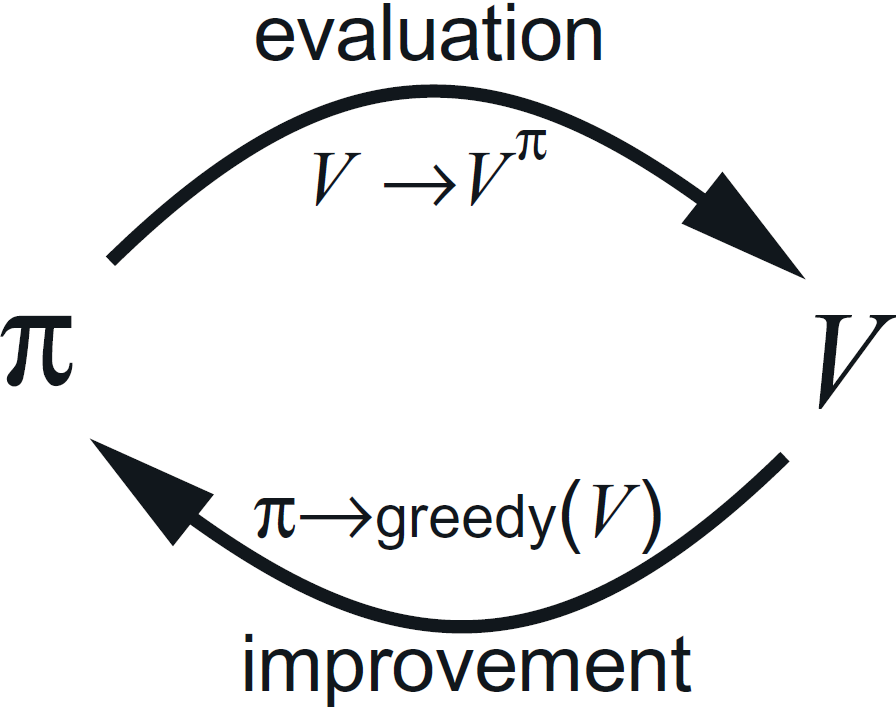
\includegraphics[width=0.35\textwidth]{pic/PI}
	\vspace{-15pt}
	\caption{Policy Iteration algorithm  \cite{sutton1998introduction}.}
	\vspace{ -15pt}
	\label{fig:PI}
\end{wrapfigure}
Notice that in this paper we discuss mostly about case of the deterministic policy. Policy Iteration(PI) and Value Iteration(VI) are the the typical algorithms to solve MDP problem. The sketch of policy iteration is shown in Figure \ref{fig:PI}. 
%Value Iteration use Bellman Equation to do the iteration, while 
PI uses equation \eqref{equ:V} in policy evaluation(PE) step until value function convergence. Policy improvement(PI) step  use Bellman Equation $\pi(s) = \arg \max_a Q(s,a)$ to update policy. PI and PE would be alternately executed until the convergence. However, for the dynamic programming(both VI and PI) we need the precise transition model and reward model. Dynamic Programming algorithm works only for discrete states and actions, otherwise we need manual discretization.

\subsection{LSTD Learning}
Temporal Difference(TD) Learning method is more widely used than DP and MC. 
%TD learning combines DP method and MC method. 
The model of the environment is not needed and the method could be either \textit{online} or \textit{offline}.
TD method aims to minimize the error of estimating Value Function $MSE(\omega) = \frac{1}{n} \sum_{i=1}^{n}(V_\omega^\pi (s_i) - V^{\pi}(s_i))^2$. The core idea is that using equation \eqref{equ:V} we get approximation of value function as $V^\pi (s_t) \approx E[r_t + \gamma V_\omega ^\pi(s_{t+1})] $. Which allows us to calculate the error MSE.  We use Stochastic Gradient Descent to To update the parameter. And the MSE is approximated by using the old approximation to get the target values for a new approximation, this behaviour is called bootstrapping.
%i.e. $MSE(\omega) \approx MSE_{BS} = \frac{1}{n}\sum_{i=1}^{n}$. 
%By comparing the prediction at the current state 
%$V_{\omega_t} (s_t)$ to the prediction of the next state $V_{\omega_t}(s_{t+1}) $ the temporal difference $\delta_t$ is used for adapting the prediction itself. 
The update rule follows,
\begin{align}
\theta ' &= \theta - \alpha \nabla MSE(\theta)\nonumber  \\
		&= \theta -[V_\theta^\pi(s_i) - V^{\pi}(s_i)] \nabla_{\theta_t}V_{\theta_t} (s_t) \nonumber \\
		&= \theta + \alpha \delta_t \nabla_{\theta_t} V_{\theta_t}(s_t),
% \delta_t &= r_{t} + \gamma V_{\theta_t}(s_{t+1}) - V_{\theta_t}(s_t) \nonumber
\end{align}
where $\delta_t$ is the TD error and it is defined as $\delta_t = r_{t} + \gamma V_{\theta_t}(s_{t+1}) - V_{\theta_t}(s_t)$.
%Note that  we actually ignore the gradient  of term $V^\pi_\theta(s_{t+1})$ by updating the parameters. \\
To speed up the process of reward propagation, eligibility traces could be used \cite{boyan1999least}. 
If we approximate action-value function Q(s, a) instead of state-value function V(s), it leads to Q-Learning and SARSA. The update rule follows: 
\begin{align}
\theta ' &= \theta + \alpha \delta_t \nabla_{\theta_t} Q_{\theta_t}(s_t, a_t) \label{equ:Q:learn}\\
\delta_t &= r_{t} + \gamma Q_{\theta_t}(s_{t+1}, a_{?}) - Q_{\theta_t}(s_t, a_t) \label{equ:Q:learn2},
\end{align}
where $a_{?}$ could be $\arg\max_a Q(s_t+1, a)$ (Q-Learning) or $a_{t+1}$ (SARSA). Those two algorithms are also standard TD learning methods..
\subsection{Linear Function Approximation and kernel Methods } %
For approximation of value function, linear function approximators are commonly used. Introducing a feature vector $\phi(s)$, holding linear basis functions, and a parameter vector $\theta$,
used to align the functions, the value function can be approximated as  $V(s) \approx V_\theta (s) = \theta^T \phi (s)$\\
 Where $\omega$ is a set of weights(parameters). We could use batch of data to minimize the TD error to increase data efficiency and least approximation could directly give the closed form solution. Recall the problem
$\min_\omega MSE_{BS}(\omega) = \frac{1}{n} \sum_{i=1}^{N}(r(s_i, a_i) + \gamma Q_{\omega_{old}} (s_i'. a_i') - Q_\omega (s_i, a_i) )^2$. We could directly get closed form LSTD solution: $\omega = (\vec{\Phi}^T \vec\Phi)^{-1}\vecPhi(R+\gamma\vecPhi' \omega_{old})$. 
\\
Kernel methods is also widely used in linear regression, which supplies a non-parametric methods.  LSTD algorithm is actually a linear regression problem. Thus we could use kernel method to solve this problem. According to the Mercer theorem \cite{vapnik1999overview}, there exists a Hilbert space H and a mapping $\phi$ from S to H such that $k(s_i, s_j) = \langle \phi(s_i), \phi(s_j) \rangle$. This yield kernel trick, we could directly calculate the inner product instead of calculating feature of $s_i$ and $s_j$ individually although H could be even infinite dimensional and do not need to know or design $\phi$. 



\section{Method}
\subsection{LSPI Method}
We linearly approximate $Q(s, a) = \omega^T \phi (s, a) = \sum_{i=1}^k \phi_i (s, a) \omega_i $. Recall that the state-action value function $Q^\pi$ is the solution of Bellman Equation, $Q^\pi(s, a) = r(s, a) + \gamma \sum_{s'} \sum_{a'} P(s' \vert a, s) \pi(a' \vert s') Q^\pi(s', a')$. We could rewrite it as 
$Q^\pi = R^\pi + \gamma \vec{P}^\pi Q^\pi$. Where $Q^\pi$ and $R^\pi$ are vectors of size$\vert S \vert \vert A \vert$ and $\vec{P}^\pi$ is the stochastic transition matrix of size $\vert S \vert \vert A \vert \times \vert S \vert \vert A \vert$, which describes the transitions from pair (s, a) to pair $(s', \pi (s') )$.  With Linear Approximation, we rewrite the equation as \\
\begin{align}
\vec \Phi \omega &\approx R^\pi + \gamma \vec{P}^\pi \vecPhi \omega\\
(\vec \Phi - \gamma \vec{P}^\pi \vecPhi) \omega &\approx R^\pi ,
\end{align}
where $\vec \Phi = ( \phi(s_1, a_1), ..., \phi(s, a), ..., \phi(s_{\vert S \vert}, a_{\vert A \vert}))^T$, P and $R^\pi$ are defined as before. We are interested in a set of weights $w$ that yields a fixed point in value function space, that a value function $Q(s, a) = \omega^T \phi (s, a)$ is invariant under one step of value determination followed by orthogonal projection to the space spanned by the basis functions\cite{lagoudakis2003least}. Assuming that the columns of $\vecPhi$ are linearly independent:
\begin{align}
\vecPhi ( \vecPhi^T \vecPhi)^{-1}\vecPhi^T (R^\pi + \gamma \vec{P} ^{\pi}\vecPhi \omega) = \vecPhi \omega \Rightarrow \vecPhi^T (\vec \Phi - \gamma \vec{P}^\pi \vecPhi) \omega = \vecPhi^T R^\pi \label{equ:Aw=b}
\end{align}
From equation \eqref{equ:Aw=b} we could construct the form of $\vec A \omega = \vec{b}$, where $\vec{A} =\vecPhi^T (\vec \Phi - \gamma \vec{P}^\pi \vecPhi), \vec{b} = \vecPhi^T R^\pi$. The matrix $\vec{P}^\pi$ requires the model of system. However, we could use the samples to approximate the term $\vec{A}$ and $\vec{b}$. $\vec{\Phi}= ( \phi(s_1, a_1), ..., \phi(s, a), ..., \phi(s_n, a_n) )^T, \vec{P}\pi \vecPhi = $ $ \vec  ( \phi(s_1', \pi(s_1')), ..., $ $\phi(s', \pi(s')), ..., $ \\ $\phi(s'_{n}, \pi(s'_{n})))^T, R = (r(s_1, a_1), ..., r(s, a), ..., r(s_n, a_n)))$. 
%We could also use (s', a') to approximate $P\vec\Phi$.
Normally we write it as additive form as is shown in Algorithm 2. This algorithm is called LSQ, since it's similar to LSTD. We combined LSQ and Policy Iteration, using LSQ as policy evaluation and using Equation $\pi(s) = \arg\max_a Q(s,a)$ as policy improvement, we get the algorithm least square policy iteration (LSPI). The algorithm is shown as follows:  \\
\noindent
\begin{minipage}[c]{0.45\linewidth}
	\begin{algorithm}[H]
	\caption{LSPI}
	\label{alg:LSPI}
	\begin{algorithmic}
		\STATE {\textbf{Input} D, $\phi$, $\gamma$ $\pi_0$} 
		\STATE {// D: Dataset of samples}
		\STATE {// $\phi$: Basis function}
		\STATE {// $\pi_0$: initial policy}
		\REPEAT 
		\STATE {update D (optional)}
		\STATE {$\pi \leftarrow \pi'$}
		\STATE {$\pi' \leftarrow $  LSTDQ $(D, \phi, \gamma, \pi)$}
		
		\UNTIL{$\pi$ convergence}
	\end{algorithmic}
\end{algorithm}
\end{minipage}
\begin{minipage}[c]{0.51\linewidth}
		\begin{algorithm}[H]
	\caption{LSTDQ}
	\label{alg:LSTDQ}
	\begin{algorithmic}
		\STATE {\textbf{Input} D, $\phi$, $\gamma$ $\pi$} \\
		\STATE {A $\leftarrow$ 0}
		\STATE {b $\leftarrow$ 0}\\ 
		
		\FOR{ each $(s, a, s', r) \in D$ }
		\STATE { $A \leftarrow A + \phi(s, a)(\phi(s, a) - \gamma \phi(s', \pi(s')))^T$}
		\STATE { b $\leftarrow$ b + $\phi(s,a)r$}
		\ENDFOR		
		\STATE { $\omega^\pi \rightarrow A^{-1}b$}
		
		\RETURN { $\omega^\pi$}	
		
	\end{algorithmic}
\end{algorithm}
\end{minipage}
\\
\\
\noindent
If there is absorbing states in Markov chains, feature of those states should be zeros. The update rule would then become $A_k:=A_{k-1} + \phi(s, a)(\phi(s, a) - 0)^T$.\\
The choice of basis function is a fundamental problem. Normally we would use polynomial feature, radial basis function. Recently there are also some successful result on application of random Fourier features into reinforcement learning problem \cite{rahimi2008random}\cite{rajeswaran2017towards}. \\
The numerical stability is also an important issue. In LSTDQ algorithm, we need to calculate inverse of matrix A, however, A could not always be full rank. A practical trick is use ridge regression $(A + \lambda I)^{-1} b$, $\lambda$ is a small number to enhance the numerical stability. It could also be regarded as a regularized regression problem. There are also some other algorithm using regularization to improve LSTD process such like \textit{l2}-regularization, LARS-TD \cite{kolter2009regularization}\cite{petrik2010feature}. Also we could use some methods to compute the inverse of A such like singular value decomposition(SVD) or using Sherman-Morrison formula to compute inverse matrix implicitly, which yields algorithm LSTDQ-OPT \cite{lagoudakis2003least}.
\\
LSPI gives  great flexibility in collection of samples. The sample could be collected from arbitrary policy. But an issue is that the dataset should be sufficiently representative, this is also a general exploration problem of reinforcement learning. LSPI is normally regarded as an \textit{off-line} algorithm, however, on-line version is also possible \cite{li2009online}\cite{ma2010convergence} as is shown in Algorithm 1, update the dataset is possible. LSPI is a model free algorithm, but if we have the model, we could use the model to compute the state transition matrix $P\pi$ instead of approximating $P^\pi \vecPhi$. \\
\subsection{KLSPI Method}
The design and selection of feature highly influence the performance of learning process. Good basis functions could greatly contribute to the convergence and performance. This is still a fundamental open problem in  LSPI. There are many research about improvement of feature selection for LSTD method such like NPDP, KLSPI, OSKTD, GPDP, KBPS, RKRL \cite{chen2013online}\cite{kroemer2011non}. In this paper we mainly focus on KLSPI algorithm.\\
If the feature function satisfies Mercer's Condition \cite{vapnik1999overview}, we can directly calculate kernel -- inner product of feature. According to Equation \eqref{equ:Aw=b}, we could approximate the action value function as a kernelized form:
\begin{align}
 \omega &= A^{-1} b,\\
   Q(s, a) &= \phi^T (s, a) \omega \\ 
   \Rightarrow \omega &= \vec{k} (x) ( \vec K - \gamma \vec K_P) R \\ 
   &= \alpha ^T \vec{k} (x) \label{equ:kenelQ},
\end{align}
\\
where x is the combined feature vector of state-action pair (s, a),  $\vec{k(x)} =  ( k(x, x_1) ... k(x, x_{\vert D \vert}) )^T$, $\vec{K}_{ij} = k(x_i, x_j)  = \langle \phi(x_i),  \phi(x_j) \rangle$, $\vec{K}_{P, ij} = k(x_i', x_j')  $. Equation \eqref{equ:kenelQ} implies that we could directly use the dataset instead of manually design the features and use equation \eqref{equ:kenelQ} to approximate Q(s, a). Similar to Algorithm 2, we could also derive the incremental form to construct term A and b, $A_{t+1} := A_t + \vec k (x_t)( \vec k(x_t) - \gamma \vec k_t(x_t'))^T$,  $b_t := b_{t-1} + \vec k(x_t) r_t$ \\
The problem this idea is how to decrease the computation cost and guarantee the sparsity of solutions without the loss of generalization ability, which is caused by the huge size of sample dataset that we could collect thousands of samples or even more. To solve this problem, various methods for sparsifying kernel machines were studied. For instance, support vector regression use structural risk minimization principle and $e$-intensive cost function \cite{cristianini2000introduction}. In this paper, we use integrate linear dependence (ALD) analysis into LSTDQ algorithm to solve this problem. This idea has been applied in some supervised learning algorithm such like kernel recursive LS (RLS) algorithm \cite{engel2004kernel}. It is easy to extend to RL problem and provides convergence guarantees. \\
We notice that the core problem is approximate as precise as possible and keeping the size of dataset as small as possible. To solve it, the idea of ALD approach  is that, using a data dictionary as subset of whole dataset for kernel calculation, if the feature vector of a new data cannot be approximated with a predefined precision, this data would be added to that dictionary.\\
Suppose that we have the tested t-1 feature vectors of original dataset and we have already constructed the dictionary ${\rm Dic}_{t-1} = \{ \phi (x_j)\} (j =  1...k)$, The ALD condition of a new data x is tested as follows,
\begin{align}
\delta_t = \min_c \Vert \sum_{j=1}^{\vert {\rm Dic_{t-1}} \vert} c_j\phi(x_j) - \phi(x_t) \Vert^2 \le \mu, \label{equ:ALD:formlization}
\end{align}
where $\mu$ is a threshold parameter to determine the control accuracy and sparsity level. When $\mu$ is appropriately selected, the solution could be guaranteed without sacrificing much in approximation accuracy. We use kernel trick to compute the optimization solution of \eqref{equ:ALD:formlization}, which is equivalent to,
\begin{align}
\delta_t &= \min_c \{  \sum_{i,j} c_i c_j \langle \phi(x_i), \phi(x_j) \rangle - 2\sum_i c_i \langle \phi(x_i), \phi(x_t) \rangle + \langle \phi(x_t), \phi(x_t) \rangle   \} \nonumber  \\
&= \min_c \{ c^T \vec K_{t-1}c - 2c^T \vec k_{t-1}(x_t) + k(x_t, x_t)  \} \nonumber\\
\Rightarrow c_t &= \vec K_{t-1}^{-1} \vec k_{t-1}(x_t) \label{equ:ALD:c} \\
\delta_t &=  k(x_t, x_t) - \vec k_{t-1}^T(x_t) c_t. \label{equ:ALD:delta}
\end{align}
Equation \eqref{equ:ALD:c} and \eqref{equ:ALD:delta} give the key step of ALD analysis, if $\delta_t$ is smaller than the precision threshold $\mu$, we regard as the data in dictionary is sufficient to represent and we keep the dictionary unchanged. Otherwise we add the new data $x_t$ to dictionary  $ {\rm Dic_t = Dic_{t-1} }\cup \{x_t\} $. \\
Based on the previous discussion, we combine ALD analysis and LSPI algorithm to come up KLSPI algorithm. We modifies the LSTDQ algorithm and integrate ALD analysis into LSTDQ  framework, we firstly enumerate all the state-action pair in the dataset and perform ALD analysis to construct the dictionary, then we solve the regression problem $ A \alpha = b$ as LSTDQ. The other steps are identical to LSPI algorithm. KLTDQ is described  as follows.\\


\begin{algorithm}[H]
\caption{KLSTDQ}
\label{alg:KLSTDQ}
\begin{algorithmic}
	\STATE {\textbf{Input} D, $\vec{k}$, $\gamma$ $\pi_0$, $\mu$,} 
	\STATE {// $\vec{k}$, kernel function $\vec{k}(\cdot, \cdot )$}
	\STATE {// $\mu$, threshold parameter for kernel sparsification}\\ 
%	\STATE {}
	\STATE {$\rm Dic_0 = \emptyset$, t=0}
	\FOR {each $x = (s, a) \in D$}
	\STATE {$c_t = K_{t-1}^{-1} k_{t-1}(x)$}
	\STATE {$\delta_t = k(x, x) - k_{t-1}^T(x) c_t$}
	\IF {$\delta_t<\mu$}
	\STATE { t $\leftarrow$ t+1, $\rm Dic_t \leftarrow Dic_{t-1} \cup \{x\}$}
	\ENDIF
	\ENDFOR		
	\FOR{ each $(s, a, s', r) \in D, x = (s, a), x' = (s, \pi(s'))$ }
	\STATE { $A \leftarrow A + k(x)(k(x) - \gamma k(x'))^T$}
	\STATE { b $\leftarrow$ b + $k(x) r$}
	\ENDFOR		
	\STATE { $\alpha^\pi \leftarrow A^{-1}b$}	
	\RETURN { $\alpha^\pi$}		
\end{algorithmic}
\end{algorithm}
\noindent
Like LSTD, for absorbing states in Markov chain, feature vector should be all zeros and the update rule of matrix A should be $A_{t+1} := A_t + \vec k(x) (\vec k(x) - 0 )^T$. \cite{xu2007kernel} gives the analysis and proof of convergence. KLSPI could converge to a suboptimal policy.\\
KLSPI is a very efficient non-parametric methods among TD mehods. Using ALD analysis, it could significantly decrease the size matrix without loss of generalization ability.

\section{Conclusion}
LSPI algorithm is a model-free, off-line reinforcement learning algorithm for control problem. LSPI combines the advantages of policy iteration and LSTD methods -- the policy search efficiency and data efficiency. It is very practical in control problem. However, there are still some issues to be concerned such like feature selection, numerical stability, data sampling. Feature selection is a fundamental problem among them. There are various research for feature engineering of LSTD.  KLSPI uses ALD analysis and kernel method to try to solve the problem of feature selection. The idea is borrowed from sparse kernel machine research. It is a non-parametric, data-efficient approach. 





  \newpage
%\begin{acknowledgements}
%If you'd like to thank anyone, place your comments here
%and remove the percent signs.
%\end{acknowledgements}

% BibTeX users please use one of
%\bibliographystyle{spbasic}      % basic style, author-year citations
\bibliographystyle{spmpsci}      % mathematics and physical sciences
%\bibliographystyle{spphys}       % APS-like style for physics
\bibliography{References.bib}   % name your BibTeX data base

%% Non-BibTeX users please use
%\begin{thebibliography}{}
%%
%% and use \bibitem to create references. Consult the Instructions
%% for authors for reference list style.
%%
%\bibitem{RefJ}
%% Format for Journal Reference
%Author, Article title, Journal, Volume, page numbers (year)
%% Format for books
%\bibitem{RefB}
%Author, Book title, page numbers. Publisher, place (year)
%% etc
%\end{thebibliography}

\end{document}
% end of file template.tex

